
\chapter{Code MDFT\label{chpt:mdft}}

The code MDFT upon which all the development during this thesis is
based is a Fortran 95 sequential code developed by Maximilien Levesque,
Daniel Borgis \textit{et al.} \textcolor{red}{{[}ref{]}}, which implement
the \acs{MDFT} theory. It reads the force field (pair potential)
$u(\mathbf{r},\mathbf{\Omega})$ describing the solute and the solvent
as input, as well as necessary parameters like the temperature $T$,
number density of solvent $n_{0}$, etc. It minimizes the functional
and gives the equilibrium density $\rho(\mathbf{r},\mathbf{\Omega})$,
then computes output properties. The main structure of the code is
shown in figure \ref{fig:code-mdft}.

\begin{figure}[h]
\begin{centering}
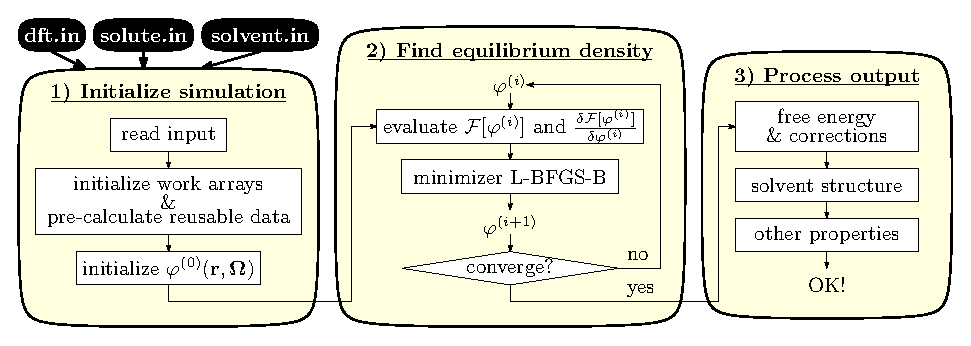
\includegraphics[width=1\columnwidth]{_figure/mdft}
\par\end{centering}
\caption{Main structure of code MDFT\label{fig:code-mdft}}
\end{figure}


\section{Supercell discretization}

$L_{x}\times L_{y}\times L_{z}$ Å$^{3}$ space is discretized on
a regular grid of $\textrm{nfft}_{1}\times\textrm{nfft}_{2}\times\textrm{nfft}_{3}$
nodes. Angular grid is discretized with Lebedev (L) or Gauss-Legendre
(GL) quadrature for $\mathbf{\Omega}\equiv\left(\Theta,\Phi\right)$,
$\Theta\in\left[0,\pi\right]$, $\Phi\in\left[0,2\pi\right]$ and
regular quadrature for $\Psi\in\left[0,\pi\right]$ as we used the
code mainly for water. The number of each angular dimension is linked
to the order of quadrature, $m_{\max}$, which is discussed mainly
in the chapter of theory.

The solute center is at $\left(\dfrac{L_{x}}{2},\dfrac{L_{y}}{2},\dfrac{L_{z}}{2}\right)$
of the box, characterized by $\mathbf{r}_{T}$. If the internal coordinates
of solute $\mathbf{r}_{M}$, the solute coordinates in the box $\mathbf{r}=\mathbf{r}_{M}+\mathbf{r}_{T}$.

\section{Minimizer L-BFGS-B}

The minimizer adopted by MDFT is the L-BFGS-B \citep{Zhu_1994_bfgs,Zhu_bfgs_1997_algorithm}
package version 3.0 written in Fortran 77, implementing the limited-memory
Broyden-Fletcher-Goldfarb-Shanno (BFGS) algorithm with constraints
of the form $l\leq x\leq u$ to the variable $x$. \textcolor{red}{During
the evaluation of the initial code which uses L-BFGS,} the constraint
function is not used.

The functional $\mathcal{F}[x_{i}]$ and the gradient of functional
$\nabla\mathcal{F}[x_{i}]=\dfrac{\delta\mathcal{F}}{\delta x}(x_{i})$
are required by L-BFGS to minimize the functional. It saves the variables
$x_{i}$ and gradient of the past $m$ iterations, which is a memory
eater.

The functional in MDFT to be minimized is eq. (\ref{eq:fff}), and
its gradient is
\begin{equation}
\frac{\delta\mathcal{F}[\rho]}{\delta\rho(\mathbf{r},\mathbf{\Omega})}=\beta^{-1}\ln\left(\dfrac{\rho(\mathbf{r},\mathbf{\Omega})}{\rho_{0}}\right)+V_{\mathrm{ext}}(\mathbf{r},\mathbf{\Omega})+V_{\mathrm{exc}}(\mathbf{r},\mathbf{\Omega})
\end{equation}
where $\rho_{0}$ is the angular density of bulk solvent, 
\begin{equation}
\rho_{0}=\left\{ \begin{array}{ll}
n_{0} & \mbox{if atomic, }\Omega\equiv1\\
n_{0}/4\pi & \mbox{if linear, }\Omega\equiv(\Theta,\Phi)\\
n_{0}/8\pi^{2} & \mbox{if non-linear, }\Omega\equiv(\Theta,\Phi,\Psi)
\end{array}\right.\label{eq:rho}
\end{equation}


\section{Treatment to avoid unphysical density}

During minimization, the density variable $\rho(\mathbf{r},\mathbf{\Omega})$
can have unphysical negative numbers, \textcolor{red}{which also cause
the divergence of the minimization.} To avoid this phenomenon, a normalized
$\varphi(\mathbf{r},\mathbf{\Omega})$ is used as the variable during
the minimization in place of $\rho(\mathbf{r},\mathbf{\Omega})$,
so that:
\begin{equation}
\rho(\mathbf{r},\mathbf{\Omega})=\rho_{0}\varphi^{2}(\mathbf{r},\mathbf{\Omega})\label{eq:cg_vect}
\end{equation}

According to the definition (\ref{eq:cg_vect}), we see:
\begin{equation}
\frac{\delta\rho(\mathbf{r},\mathbf{\Omega})}{\delta\varphi}=2\rho_{0}\varphi(\mathbf{r},\mathbf{\Omega})
\end{equation}
Therefore the gradient to feed the L-BFGS minimizer is:
\begin{equation}
\frac{\delta\mathcal{F}}{\delta\varphi}=\frac{\delta\mathcal{F}}{\delta\rho}\cdot\frac{\delta\rho}{\delta\varphi}=2\rho_{0}\varphi(\mathbf{r},\mathbf{\Omega})\cdot\left[\beta^{-1}\ln\varphi^{2}+V_{\mathrm{ext}}+V_{\mathrm{exc}}\right]
\end{equation}

